% Supplementary material for the JFM Rapids paper "A spectral theory for turbulent burning velocity across scales".
% Figures: figures/supp_*.pdf, generated by make_figures.ipynb (numbers below are from its printed output).
% On Overleaf, add this file and the supp_*.pdf figures to the paper's project and compile it as the main document
% (Menu > Main document); it uses the paper's jfm.bst and jfm.bib.

\documentclass[11pt]{article}
\usepackage[a4paper, margin=25mm]{geometry}
\usepackage{graphicx}
\usepackage{newtxtext}
\usepackage{newtxmath}
\usepackage{natbib}
\usepackage{booktabs}
\usepackage{hyperref}
\hypersetup{
    colorlinks = true,
    urlcolor   = blue,
    citecolor  = black,
    linkcolor  = black,
}
\graphicspath{{figures/}{./}}

% numbering S1, S2, ...
\renewcommand{\thesection}{S\arabic{section}}
\renewcommand{\thefigure}{S\arabic{figure}}
\renewcommand{\thetable}{S\arabic{table}}
\renewcommand{\theequation}{S\arabic{equation}}

% notation, as in the paper
\providecommand{\Rey}{\mbox{\textit{Re}}}
\providecommand{\Ka}{\mbox{\textit{Ka}}}
\newcommand{\Sct}{\mbox{\textit{Sc}}_{\, T}}
\newcommand{\sL}{s_L}
\newcommand{\dL}{\delta_L}
\newcommand{\De}{D_e^{+}}
\newcommand{\up}{u^{\prime}}

\title{Supplementary material for\\ \textit{A spectral theory for turbulent burning velocity across scales}}
\author{M. D. Walker, G. V. Nivarti, M. E. Mueller, R. S. Cant and S. Hochgreb}
\date{}

\begin{document}
\maketitle

This document accompanies the paper. Sections, figures, tables and equations numbered with the prefix S belong to this document; all other references are to the paper. The figures are produced by the notebook \texttt{make\_figures.ipynb} from the same data as the figures of the paper.

%=====================================================================
\section{Distribution of the wrinkling exponent}\label{sec:beta}

The paper connects its burning-velocity relation with the power-law wrinkling factor of \citet{Charlette2002a} for an exponent $\beta_w = 1/2$. \citet{Charlette2002b} determined $\beta_w$ locally with a dynamic procedure, and figure~\ref{fig:beta} shows the probability density function (PDF) of the exponents they obtained, digitised from figure~5 of their paper.
The digitised curve, which ends at $\beta_w = 1$, was normalised to unit area and its moments were computed by trapezoidal integration. The mean is 0.587 and the standard deviation 0.104 (variance 0.0109); the median is 0.57 and the interquartile range 0.51--0.65. About 22\,\% of the distribution lies below $\beta_w = 0.5$, and the digitised PDF falls to zero at $\beta_w = 0.4$, above the fractal value $\beta_w = 1/3$ that would recover Damk\"ohler's large-$\up$ limit $s_T \propto \up$. The distribution therefore supports an exponent close to $1/2$, centred slightly above it.

\begin{figure}[h]
  \centering
  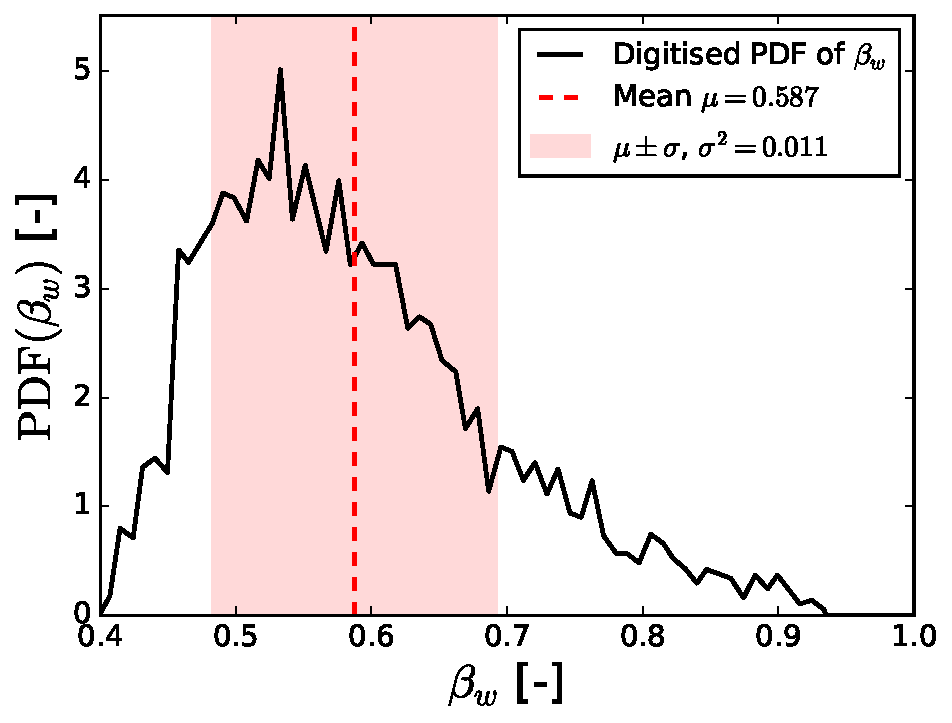
\includegraphics[width=0.6\textwidth]{supp_beta_pdf}
  \caption{PDF of the local wrinkling exponent $\beta_w$ obtained with the dynamic procedure of \citet{Charlette2002b} (digitised). Dashed line, mean $\mu = 0.587$; shading, $\mu \pm \sigma$, where $\sigma^2 = 0.011$ is the variance.}
  \label{fig:beta}
\end{figure}

%=====================================================================
\section{Selection and treatment of the experimental data}\label{sec:data}

Measured turbulent burning velocities depend on the flame configuration and on how $s_T$ is defined \citep{Driscoll2008}, so the datasets of table~1 of the paper were chosen to keep both as uniform as possible.

\subsection{Flame configuration}\label{sec:config}

\citet{Driscoll2008} groups premixed turbulent flames into envelope flames (on two-dimensional slot and axisymmetric Bunsen burners), oblique flames, unattached flat flames (on low-swirl, diffuser or counterflow burners) and spherical flames (in fan-stirred vessels). All of the datasets except Aachen are envelope flames: the Michigan (2005) flames are on a slot burner, Damk\"ohler's on tubes and the others on round Bunsen burners. The Aachen flames, on a low-swirl burner, are unattached flames in this classification.

\subsection{Turbulent burning velocity}\label{sec:sT}

In an envelope flame all of the reactants supplied by the burner pass through the flame, so mass conservation gives a mean, or global, consumption speed,
\begin{equation}
  s_T = \frac{\dot m_R}{\rho_R \bar A},
  \label{eq:consumption}
\end{equation}
where $\dot m_R$ is the mass flow rate of reactants, $\rho_R$ their density and $\bar A$ the area of a mean flame surface \citep{Filatyev2005,Driscoll2008}. Where the source reports it, $\bar A$ is taken on the isosurface $\overline{\Lambda} = 0.5$ of the mean progress variable (table~1 of the paper); for Ottawa it is $\overline{\Lambda} = 0.05$, and for Michigan (2005) it is the time-averaged flame position. Differences in equivalence ratio, within and between datasets, are accounted for by normalising $s_T$ by the laminar burning velocity $\sL$ of each mixture.

Spherically expanding flames, such as those studied at Leeds \citep{Bradley2003,Lawes2012} and Princeton \citep{Chaudhuri2012,Wu2015}, are characterised instead by a propagation or displacement speed derived from the growth rate $\mathrm{d}R / \mathrm{d}t$ of a mean flame radius $R$, often multiplied by the ratio of burned to unburned gas density. This speed increases with $R$, because a growing flame kernel is wrinkled by an increasing part of the turbulence spectrum \citep{AbdelGayed1987,Bradley2003,Lawes2012}, and \citet{Chaudhuri2012} correlated it with a Reynolds number based on the mean flame radius rather than on $\ell_0$. It measures a different quantity from (\ref{eq:consumption}), and such data are not included.

\subsection{Approaching turbulence}\label{sec:turbulence}

The approaching turbulence differs between the configurations. In an envelope flame it is generated in the burner tube or nozzle, typically by a perforated or slotted plate or a grid, and in Damk\"ohler's experiments it is the turbulence of the tube flow itself, so its spectrum is that of a turbulent pipe or nozzle flow. \citet[][figure~6.14]{Pope2000} derived the model spectrum used in the paper with one-dimensional spectra measured in a range of flows, among them turbulent pipe flow and round jets. In fan-stirred vessels the turbulence is produced by fans and is close to isotropic near the centre; its spectrum has been characterised for the Leeds vessel by \citet{AbdelGayed1987}, who measured its power spectral density, and in \citet{Walker2019}.

\subsection{Mixtures and operating conditions}\label{sec:mixtures}

To exclude differential diffusion, all of the datasets except Damk\"ohler's are methane--air flames, for which the Lewis number $\mbox{\textit{Le}} \approx 1$ \citep[e.g.][]{Kobayashi1996}, at 0.1\,MPa and about 300\,K; for this reason the high-pressure measurements of \citet{Kobayashi1996} and the propane--air flames of \citet{YuenGulder2013} are not used. Damk\"ohler's flames burned a propane--butane mixture with oxygen.

\subsection{Laminar flame thickness}\label{sec:thickness}

The sources define the laminar flame thickness differently. Michigan (2017) and Toronto (2013) give thermal thicknesses from detailed-chemistry calculations of the laminar flame (0.36\,mm, and 0.45--1.0\,mm for the flames used here); Michigan (2005) uses $\dL = 7.4 \, \alpha / \sL = 0.35$\,mm, where $\alpha$ is the thermal diffusivity of the reactants; Aachen uses $D / \sL = 0.35$\,mm with the diffusivity $D$ evaluated at 1500\,K; and the thicknesses of Tohoku and Toronto (2014), 0.066\,mm and 0.055--0.11\,mm, correspond to $\alpha / \sL$. Ottawa gives 0.033--0.065\,mm.
% TODO: state the definitions used by Ottawa and Damkohler.
The paper takes $\ell_0 / \dL$ as given by each source, or as computed from the given $\ell_0$ and $\dL$. With unity Schmidt number a consistent choice would be $\dL = \nu / \sL$, so that $\Rey = \up \ell_0 / \nu$. Reynolds numbers defined in this way, reported by the sources or computed from their tabulated $\nu$ and $\sL$, exceed those used in the paper by factors of 5.5, 6.6 and 8.9 for Michigan (2017), Toronto (2013) and Michigan (2005), and by 1.4 for Tohoku and Toronto (2014). The thickness enters the prediction only through $\mathcal{F}(\Rey)$, which varies slowly: halving or doubling $\dL$ changes the predicted $s_T$ by about 10\,\% at the median and by at most 21\,\%. Re-evaluating $\Rey$ as $\up \ell_0 / \nu$ for these five datasets changes the fraction of points within a factor of 1.5 of the prediction from 71\,\% to 69\,\%, and the r.m.s.\ logarithmic deviation from 0.38 to 0.37, although individual datasets shift: the geometric-mean ratio of measurement to prediction changes from 1.06 to 0.96 for Michigan (2017), from 1.06 to 0.74 for Toronto (2013) and from 1.37 to 1.04 for Michigan (2005).

%=====================================================================
\section{Scaling of the burning velocity with Reynolds and Karlovitz numbers}\label{sec:fan}

Figure~\ref{fig:fan} shows the measured $s_T / \sL$ divided by $\Ka$ against $\Rey$ for the eight datasets of table~1 of the paper, with the same values and symbols. The dashed lines are $100 \, \Rey^{-n}$, labelled with their slope $-n$. Since $\Ka = (\up / \sL)^{3/2} (\ell_0 / \dL)^{-1/2}$ and $\Rey = (\up / \sL)(\ell_0 / \dL)$, a series of measurements at fixed $\ell_0 / \dL$ in which $s_T / \sL \propto (\up / \sL)^m$ follows
\begin{equation}
  \frac{s_T / \sL}{\Ka} \propto \Rey^{\, m - 3/2}
  \label{eq:fan}
\end{equation}
in this plane. A slope of $-1/2$ thus corresponds to Damk\"ohler's linear scaling, $m = 1$, and a slope of $-1$ to $m = 1/2$, the strong-turbulence limit of the paper's relation $s_T / \sL = [1 + \mathcal{C} \, \mathcal{F}(\Rey) \, \up / \sL]^{1/2}$ apart from the weak variation of $\mathcal{F}$ with $\Rey$. Datasets in which $\ell_0 / \dL$ varies together with $\up / \sL$ do not follow (\ref{eq:fan}) exactly.
% TODO: check that this reading of the fan is the intended one.

\begin{figure}[h]
  \centering
  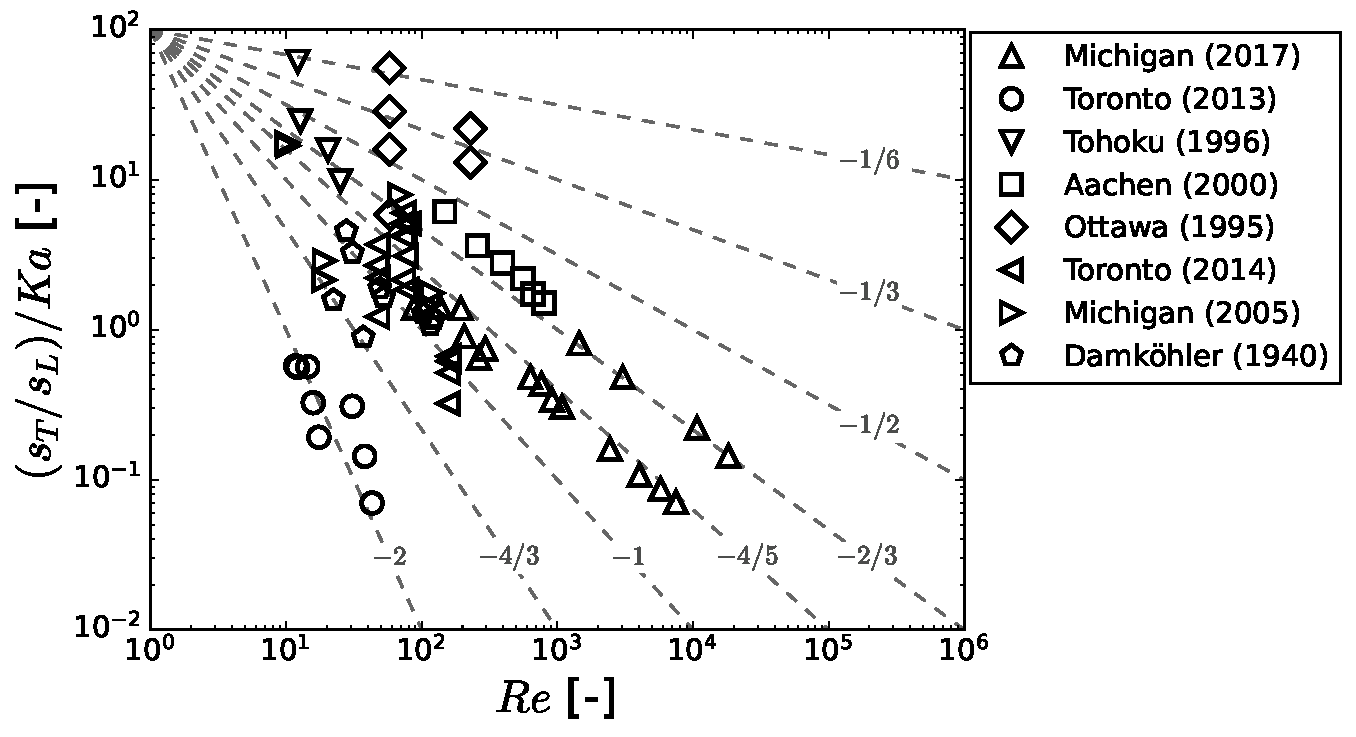
\includegraphics[width=0.8\textwidth]{supp_scaling_fan}
  \caption{Measured $s_T / \sL$ divided by $\Ka$ against $\Rey$ for the datasets of table~1 of the paper (symbols as there). Dashed lines, $100 \, \Rey^{-n}$, labelled with their slope $-n$.}
  \label{fig:fan}
\end{figure}

%=====================================================================
\section{Fits to the spectral eddy viscosity and diffusivity}\label{sec:chollet}

The functions $\nu_e^{+}(\kappa / \kappa_c)$ and $\De(\kappa / \kappa_c)$ computed by \citet{Chollet1984} were digitised for $0.01 \leqslant \kappa / \kappa_c \leqslant 1$ and fitted by nonlinear least squares with the form that \citet{Pope2000} used for $\nu_e^{+}$,
\begin{equation}
  \nu_e^{+}, \ \De = C^{-3/2} \left[A + B \exp\left(-c \, \frac{\kappa_c}{\kappa}\right)\right], \qquad C = 1.5.
  \label{eq:fit}
\end{equation}
Table~\ref{tab:fit} lists the coefficients and the values at the cusp, $\kappa = \kappa_c$, which are the values used in the paper; the turbulent Schmidt number is $\Sct = \nu_e^{+} / \De$. The fitted curves are shown in figure~2(\textit{b}) of the paper. The regression of \citet{Pope2000} for $\nu_e^{+}$ gives a cusp value 26\,\% lower than the fit to the curve of \citet{Chollet1984}.
\begin{table}[h!]
  \centering
  \begin{tabular}{lcccc}
    \toprule
                                             & $A$    & $B$   & $c$   & Value at $\kappa = \kappa_c$ \\
    \midrule
    $\nu_e^{+}$, \citet{Pope2000}            & 0.441  & 15.2  & 3.03  & 0.640 \\
    $\nu_e^{+}$, fit to \citet{Chollet1984}  & 0.4927 & 162.7 & 4.996 & 0.868 \\
    $\De$, fit to \citet{Chollet1984}        & 0.8717 & 949.5 & 5.908 & 1.88  \\
    $\Sct = \nu_e^{+} / \De$                 &        &       &       & 0.462 \\
    \bottomrule
  \end{tabular}
  \caption{Coefficients of (\ref{eq:fit}) and values at the cusp.}
  \label{tab:fit}
\end{table}

\bibliographystyle{jfm}
\bibliography{jfm}

\end{document}
